% !TeX spellcheck = en_US
%\documentclass{beamer}
\documentclass[handout]{beamer}
\usepackage[spanish]{babel}
\usepackage[utf8]{inputenc}
\usepackage{graphicx}
\usepackage{tcolorbox}
\usepackage{color}

\usepackage{braket}
\usepackage{hyperref}
%\setbeamercolor{frametitle}{fg=white}
%\usefonttheme{structuresmallcapsserif}
\setbeamertemplate{footline}[frame number]
\setbeamerfont{footnote}{size=\tiny}

\setbeamercolor{page number in head/foot}{fg=black}

\usepackage{mhchem}
\usepackage{tikz}
\def\checkmark{\tikz\fill[scale=0.4](0,.35) -- (.25,0) -- (1,.7) -- (.25,.15) -- cycle;} 

\usepackage{default}

\usepackage[backend = bibtex, style = verbose, sorting = none, autocite = footnote]{biblatex}
\addbibresource{references.bib}

\newcommand\blfootnote[1]
{%
	\begingroup
	\renewcommand\thefootnote{}\footnote{#1}%
	\addtocounter{footnote}{-1}%
	\endgroup
}
\newcommand{\fcite}[1]{\blfootnote{\cite{#1}}}

\usetheme{Berkeley}

\begin{document}
	\begin{frame}
		\centering
		%\color{white}
		\textsc{\Large Técnicas de medición de fenómenos eléctricos en superficies}
		\\
		\vspace{3cm}
		\raggedleft Juan Barbosa \\
		\raggedleft \small Fisicoqu\'imica avanzada
	\end{frame}

\begin{frame}{Contenidos}
	\tableofcontents
\end{frame}

\section{Introducci\'on}
\begin{frame}{Introducci\'on}
	\begin{itemize}
		\item \textbf{Fen\'omenos el\'ectricos:} asociados a la presencia y movimiento de materia con carga el\'ectrica.
		
		\item \textbf{Superficie:} es la capa m\'as externa de un objeto, en ella tienen lugar las interacciones del objeto con los alrededores.
	\end{itemize}

	\fcite{butt2006physics}
\end{frame}

\begin{frame}{Introducci\'on}
	\begin{itemize}
		\item Los primeros estudios se llevaron acabo usando superficies cargadas en s\'olidos.
		
		\item Distintos modelos han sido propuestos para describir las superficies cargadas.
		\begin{figure}[h]
			\centering
			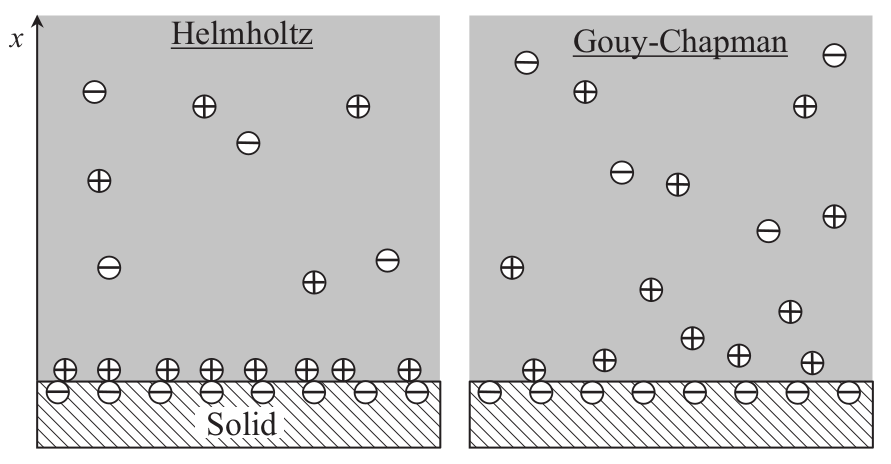
\includegraphics[width=0.5\linewidth]{sources/surfaceLiquid}
		\end{figure}
	
		\item En general, las cargas superficiales ocasionan un campo el\'ectrico, el cual atrae cargas opuestas. La capa de cargas y contraiones se denomina \textit{doble capa el\'ectrica}.
	\end{itemize}
	\fcite{butt2006physics}
\end{frame}

\begin{frame}{Introducci\'on}
	El modelo de Helmholtz es el m\'as simple de todos.
	\begin{table}[h]
		\small
		\begin{tabular}{c|p{3cm}p{3cm}}
			\textbf{Teor\'ia} & \textbf{Caracter\'isticas} & \textbf{Aproximaciones} \\
			\hline
			Helmholtz & La carga total de la superficie es neutralizada por contraiones. El potencial disminuye linealmente. & No considera el movimiento t\'ermico, difusi\'on, y adsorci\'on \\
			\hline
			Gouy-Chapman & Tiene en cuenta los movimientos t\'ermicos & Carga uniforme en la superficie, cargas puntuales \\
			\hline
		\end{tabular}
	\end{table}
\end{frame}

\begin{frame}{Estad\'istica de Boltzmann}
	\begin{equation}
		\dfrac{\braket{N_i}}{N} = \dfrac{g_i}{e^{(E_i - \mu)}/kT} \longrightarrow \left(\dfrac{g_i}{Z}\right)e^{-E_i/kT}
	\end{equation}
	Considerando el volumen total en soluci\'on, es posible asociar una distribucci\'on de concentraciones.
	
	\begin{equation}
		\dfrac{\braket{N_i}}{N}\left(\dfrac{N}{VN_A}\right) = \left(\dfrac{g_i}{Z}\right)\left(\dfrac{N}{VN_A}\right)e^{-E_i/kT}
	\end{equation}
	\begin{equation}\label{eq: c}
		\dfrac{\braket{N_i}}{VN_A} = \dfrac{n}{V} = c_i = c_{0_i}e^{-E_i/kT}
	\end{equation}
	\fcite{butt2006physics}
\end{frame}

\begin{frame}{Ecuaci\'on de Poisson}
	Describe el potencial causado por una distribucci\'on de densidad de carga o masa ($\rho$).
	\begin{equation}
		\Delta \psi = \nabla^2 \psi = -\dfrac{\rho}{\epsilon\epsilon_0}
	\end{equation}
	
	La energ\'ia corresponde con:
	\begin{equation}
		E_i = z_ie\psi \longleftarrow U = qV
	\end{equation}
	
	Usando (\ref{eq: c}) es posible obtener la densidad de carga:
	\begin{equation}
		\rho = \sum (z_ie)c_i = \sum (z_ie) c_{0_i}e^{-(z_ie)\psi/kT}
	\end{equation}
	
	El potencial el\'ectrico est\'a dado por:
	\begin{equation}
		\nabla^2 \psi = -\dfrac{\rho}{\epsilon\epsilon_0} = -\dfrac{\sum (z_ie) c_{0_i}e^{-(z_ie)\psi/kT}}{\epsilon\epsilon_0}
	\end{equation}
\end{frame}

\begin{frame}{Ecuaci\'on de Poisson}
	Para un cati\'on y ani\'on monovalentes:
	\begin{equation}
		\nabla^2 \psi = -\dfrac{e c_{0}e^{-e\psi/kT} - e c_{0}e^{e\psi/kT}}{\epsilon\epsilon_0}
	\end{equation}
	\begin{equation}
		\nabla^2 \psi(x, y, z) = \dfrac{ec_0}{\epsilon\epsilon_0} \left(e^{e\psi(x, y, z)/kT} -e^{-e\psi(x, y, z)/kT}\right)
	\end{equation}
	
	\begin{itemize}
		\item La ecuaci\'on anterior corresponde con la ecuaci\'on de Poisson-Boltzmann y en la mayor\'ia de los casos debe ser resuelta num\'ericamente.
		
		\item Describe matem\'aticamente una doble capa el\'ectrica.
	\end{itemize}
\end{frame}

\begin{frame}{}
	Existen m\'ultiples t\'ecnicas para medir las propiedades de dobles capas el\'ectricas.
	\begin{itemize}
		\item \textbf{Electrocapilaridad:} tensi\'on interfacial en funci\'on del potencial de una superficie met\'alica.
		\item \textbf{Capacitancia:} permiten determinar las densidades de carga superficiales.
		\item \textbf{Fuerzas en la superficie:} determinar la dependencia de la doble capa el\'ectrica con la distancia.
	\end{itemize}
	\fcite{butt2006physics}
\end{frame}

\section{Electrocapilaridad}
\begin{frame}{Electrocapilaridad}
	\begin{columns}
		\begin{column}{0.4\textwidth}
			\begin{figure}[h]
				\centering
				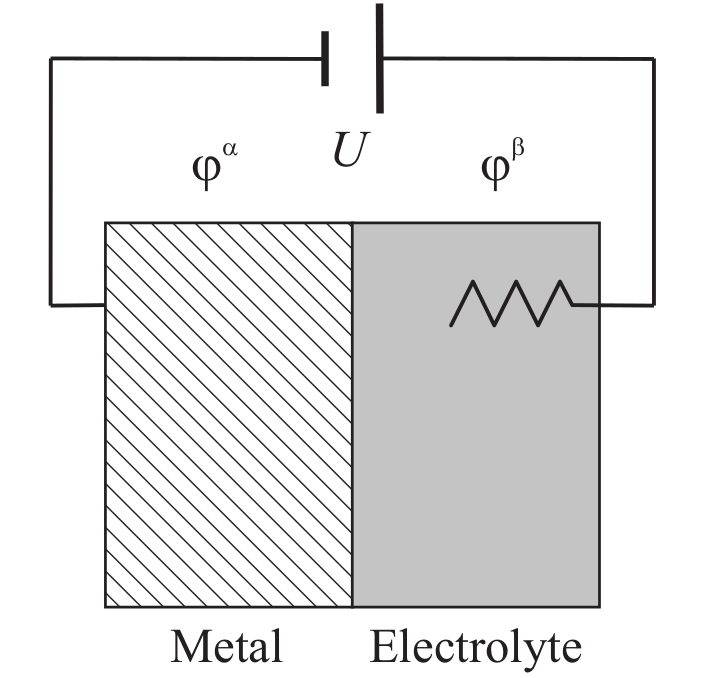
\includegraphics[width=\linewidth]{sources/electrocapillarity}
			\end{figure}
		\end{column}
		\begin{column}{0.6\textwidth}
			\begin{itemize}
				\item Permite obtener informaci\'on detallada de la doble capa el\'ectrica.
				\item El cambio en la tensi\'on interfacial, entre un metal/electrolito, se determina al cambiar un potencial aplicado.
			\end{itemize}
		\end{column}
	\end{columns}
	\fcite{butt2006physics}
\end{frame}

\begin{frame}{Electrocapilaridad}
	\small
	\begin{columns}
		\begin{column}{0.6\textwidth}
			\begin{equation}\label{eq: gd}
				d\gamma = -\sum\limits_{i=1}^n\Gamma_id\mu_i^* - \Gamma_ed\mu_e^*
			\end{equation}
			\begin{equation}\label{eq: mu}
				d\mu_j^* = d\mu_j + Z_jF_Ad\psi
			\end{equation}
		\end{column}
		\begin{column}{0.4\textwidth}
			\begin{itemize}
				\item $\Gamma_i = N_i/A$, Concentraci\'on de exceso interfacial del ion $i$.
				\item $\mu_i$ potenciales qu\'imico, y $\mu_i^*$ electroqu\'imico del ion $i$.
				\item $Z_i$ carga del ion $i$.
				\item $\psi$ potencial el\'ectrico.
			\end{itemize}
		\end{column}
	\end{columns}

	\begin{equation}
		\sum\limits_{i=1}^n\Gamma_id\mu_i^* = \sum\limits_{i=1}^n\Gamma_i(d\mu_i + Z_iF_Ad\psi) = \sum\limits_{i=1}^n\Gamma_id\mu_i + \sum\limits_{i=1}^n\Gamma_iZ_iF_Ad\psi
	\end{equation}
	\fcite{butt2006physics}
\end{frame}

\begin{frame}{Electrocapilaridad}
	\small
	\begin{equation}
		d\gamma = -\sum\limits_{i=1}^n\Gamma_id\mu_i - F_A\sum\limits_{i=1}^n\Gamma_iZ_id\psi - \Gamma_ed\mu_e + F_A\Gamma_ed\psi
	\end{equation}
	Se consideran ahora dos potenciales, uno por cada fase $\alpha\rightarrow$ metal y $\beta\rightarrow$ l\'iquido.
	\begin{equation}
		d\gamma = -\sum\limits_{i=1}^n\Gamma_id\mu_i - F_A\sum\limits_{i=1}^n\Gamma_iZ_id\psi^\beta - \Gamma_ed\mu_e + F_A\Gamma_ed\psi^\alpha
	\end{equation}
	
	El sistema se considera el\'ectricamente neutro.
	\begin{equation}
		\sum\limits_{i=1}^n\Gamma_iZ_i = \Gamma_e
	\end{equation}
	\fcite{butt2006physics}
\end{frame}

\begin{frame}{Electrocapilaridad}
	\small
	\begin{equation}
		d\gamma = -\sum\limits_{i=1}^n\Gamma_id\mu_i - F_A\sum\limits_{i=1}^n\Gamma_iZ_id\psi^\beta - \Gamma_ed\mu_e + F_A\sum\limits_{i=1}^n\Gamma_iZ_id\psi^\alpha
	\end{equation}
	
	\begin{equation}
		d\gamma = -\sum\limits_{i=1}^n\Gamma_id\mu_i - \Gamma_ed\mu_e - F_A\sum\limits_{i=1}^n\Gamma_iZ_id(\psi^\beta + \psi^\alpha)
	\end{equation}

	\begin{equation}
		d\gamma = -\sum\limits_{i=1}^n\Gamma_id\mu_i - \Gamma_ed\mu_e - \sigma d(\psi^\beta + \psi^\alpha)
	\end{equation}
	
	\begin{equation}
		\dfrac{d\gamma}{d(\psi^\beta + \psi^\alpha)} = \dfrac{d\gamma}{dU} = -\sigma = \dfrac{\gamma}{U}
	\end{equation}
	
	Donde $\sigma$ corresponde con la densidad superficial de carga.	
	\fcite{butt2006physics}
\end{frame}

\begin{frame}{Electrocapilaridad}
	\small
	Para un capacitor:
	\begin{equation}
		C = \dfrac{Q}{V} = \dfrac{dQ}{dV}
	\end{equation}
	\begin{equation}
		\dfrac{C}{A} = C^A = \dfrac{dQ/dA}{dU} = \dfrac{d\sigma}{dU} = -\dfrac{d^2\gamma}{dU^2}
	\end{equation}
	
	Experimentalmente se tiene:
	\begin{equation}
		\int\limits_{\gamma_0}^{\gamma}d\gamma = \int\limits_{0}^{U}\left(\dfrac{d\gamma}{dU'}\right)dU' = \int\limits_{0}^{U}-\sigma dU' = \int\limits_{0}^{U}-C^AU'dU' = -\dfrac{1}{2}C^AU^2 
	\end{equation}
	\begin{equation}
		\gamma = \gamma_0 - \dfrac{1}{2}C^AU^2
	\end{equation}
	\fcite{butt2006physics}
\end{frame}

\begin{frame}{Electrocapilaridad}
	\begin{columns}
		\begin{column}{0.6\textwidth}
			\begin{figure}[h]
				\centering
				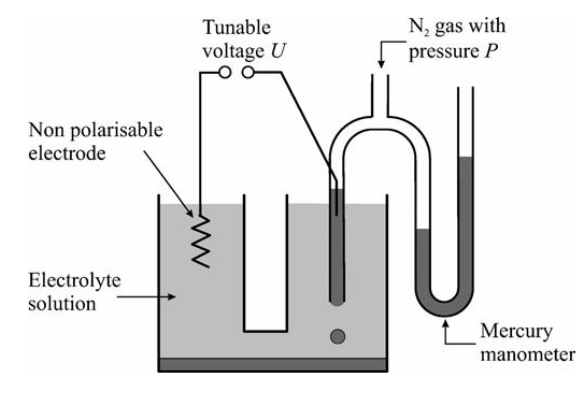
\includegraphics[width=0.7\linewidth]{sources/electro}
			\end{figure}
		\end{column}
		\begin{column}{0.4\textwidth}
			\begin{figure}[h]
				\centering
				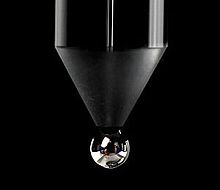
\includegraphics[width=0.7\linewidth]{sources/dropping}
			\end{figure}
		\end{column}
	\end{columns}
	\begin{figure}[h]
		\centering
		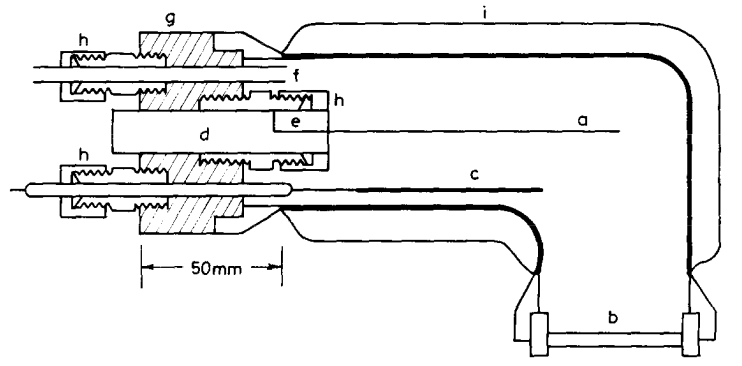
\includegraphics[width=0.5\linewidth]{sources/solidElectro}
	\end{figure}
	\fcite{butt2006physics}
	\fcite{fredlein1974electrocapillary}
\end{frame}

\section{Capacitancia}
\begin{frame}{Cronoamperometr\'ia}
	\begin{columns}
		\begin{column}{0.4\textwidth}
			\begin{figure}[h]
				\centering
				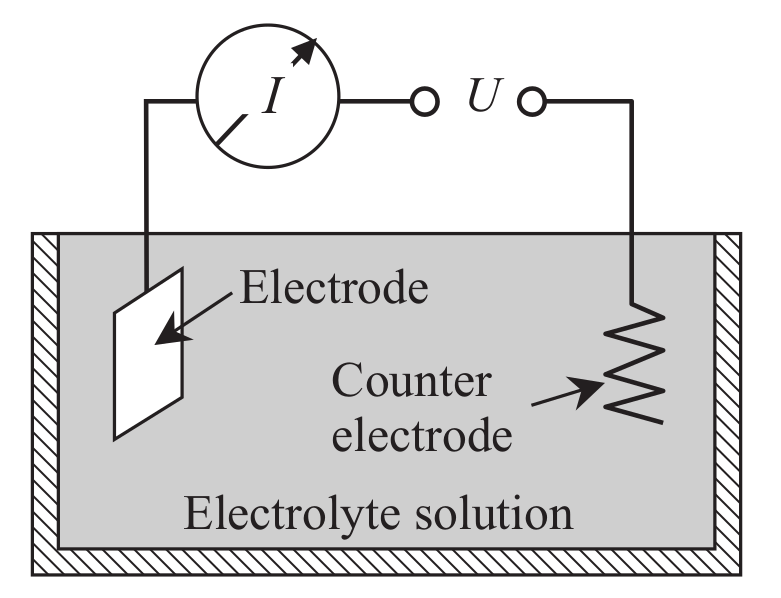
\includegraphics[width=\linewidth]{sources/capacitance}
				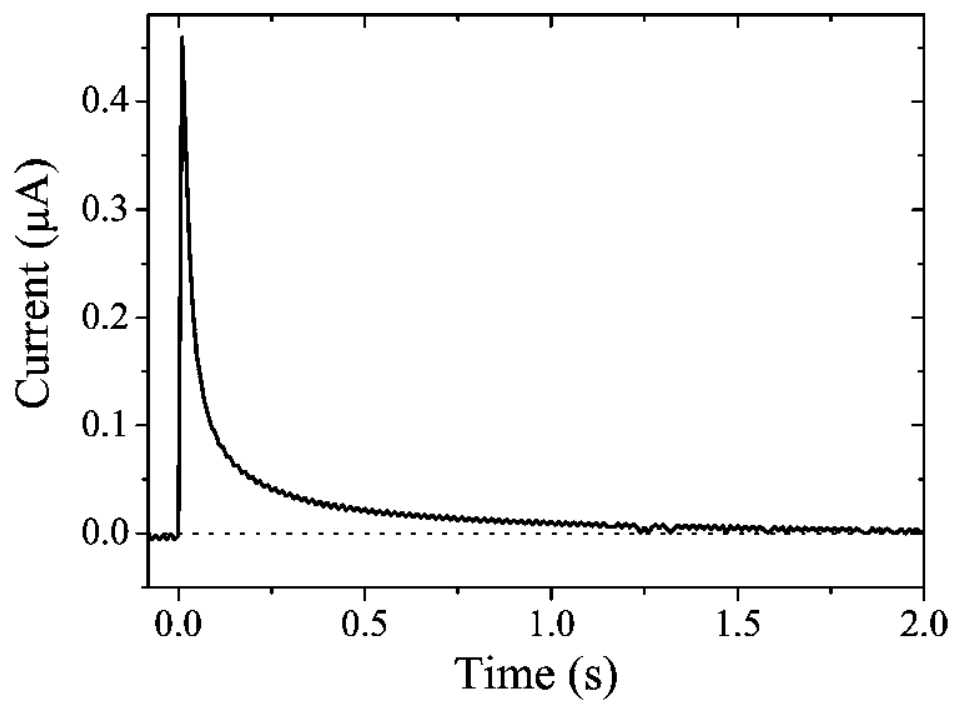
\includegraphics[width=\linewidth]{sources/crono}
			\end{figure}
		\end{column}
		\begin{column}{0.6\textwidth}
			Permite obtener el valor de capacitancia para una interface.
			\begin{equation}
				I = I(t) = \dfrac{Q}{t} = \dfrac{dQ}{dt}
			\end{equation}
			\begin{equation}
				\int\limits_{0}^{t} I(t')dt' = \int\limits_{0}^{t}\dfrac{dQ}{dt'}dt' = Q
			\end{equation}
			\begin{equation}
				C = \dfrac{Q}{U} \longrightarrow \sigma = \dfrac{Q}{A}
			\end{equation}
		\end{column}
	\end{columns}
	\fcite{butt2006physics}
\end{frame}

\section{Fuerzas en la superficie (AFM)}
\begin{frame}{Fuerzas en la superficie (AFM)}
	\begin{columns}
		\begin{column}{0.6\textwidth}
			\begin{figure}[h]
				\centering
				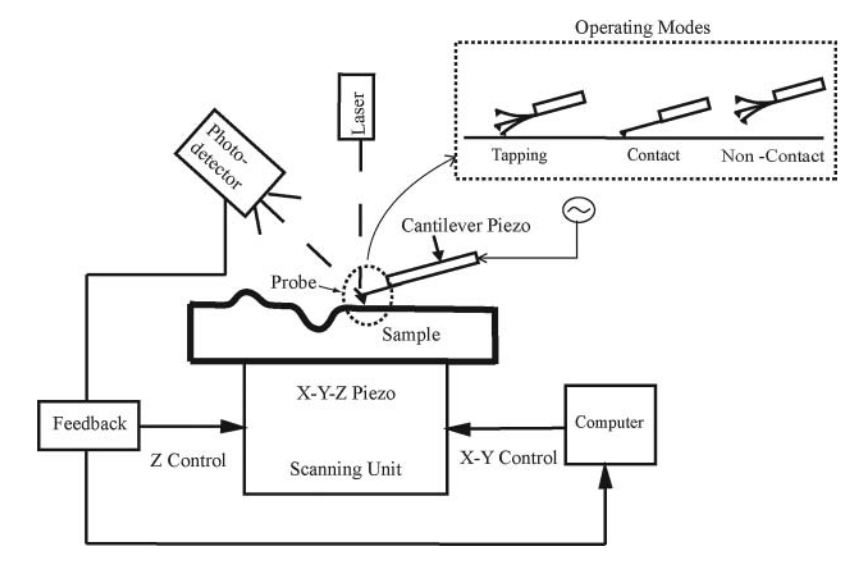
\includegraphics[width=\linewidth]{sources/afm}
			\end{figure}
		\end{column}
		\begin{column}{0.4\textwidth}
			\begin{itemize}
				\item Desarrollado por Gerd Binning y colaboradores en 1985.
				\item Una punta conductora puede actuar como un electrodo m\'ovil.
			\end{itemize}
		\end{column}
	\end{columns}
	\fcite{avila2010electrical}
\end{frame}

\begin{frame}{Fuerzas en la superficie (AFM)}
	\begin{figure}[h]
		\centering
		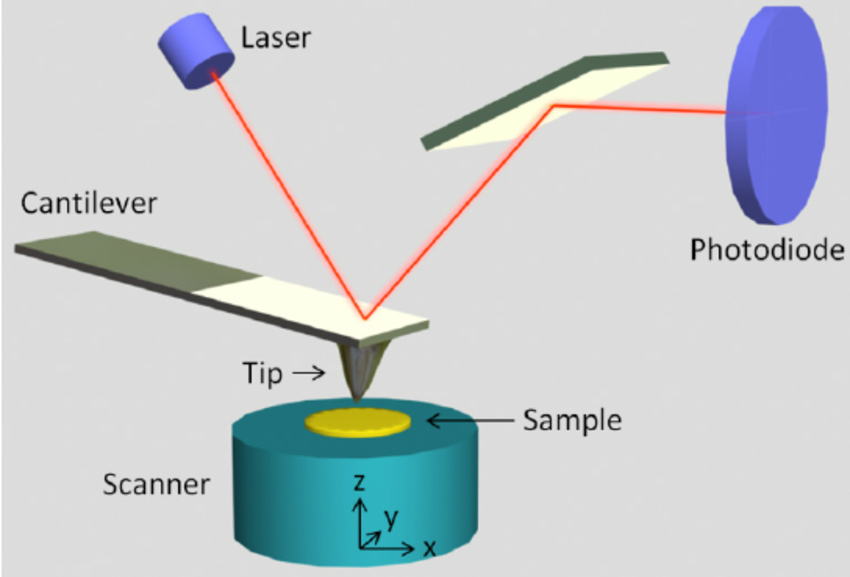
\includegraphics[width=0.7\linewidth]{sources/afmb}
	\end{figure}
\end{frame}

\begin{frame}{Fuerzas en la superficie (AFM)}
	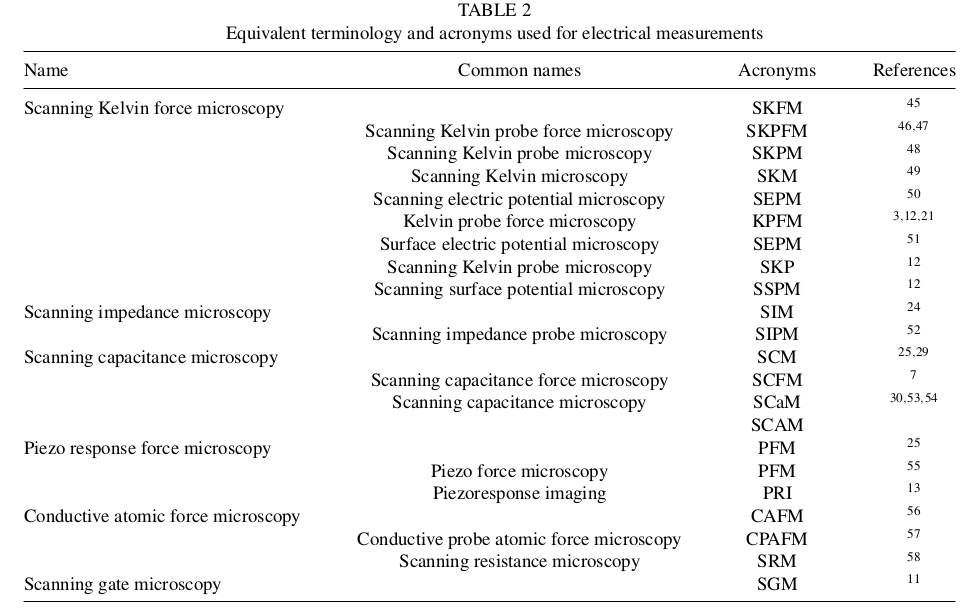
\includegraphics[width=0.9\linewidth]{sources/afm1}
	\fcite{avila2010electrical}
\end{frame}

\begin{frame}{Electrostatic force microscopy (EFM)}
	\begin{figure}[h]
		\centering
		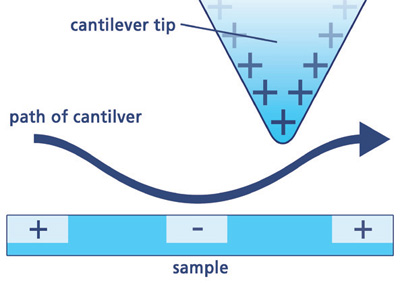
\includegraphics[width=0.7\linewidth]{sources/efm}
	\end{figure}
	\begin{equation}
		F = \dfrac{1}{2}\dfrac{\partial C}{\partial z}\Delta V^2
	\end{equation}
	\fcite{avila2010electrical}
\end{frame}



%\section{Conclusiones}
%\begin{frame}{Conclusiones}
%\end{frame}

\end{document}